%!TEX root = ../master.tex
\chapter{Background Research}\label{ch:bgresearch}



\section{Types of sources}\label{sec:typesofsources} 
The sources used in this chapter include scientific articles regarding the topic “Image to sound conversion”. The articles are published in the fields of physics, sound art and digital media. Other sources include recorded lectures of one of the articles authors.

\section{Previous work}\label{sec:previouswork}

\subsection{An experimental system for auditory image representation}\label{sec:experimentalsystem}
\todo{make introduction, then go into blindess}
(victors) To interpret an image, it is commonly the visual aspect which has the major role of deciphering what the human eyes can see. However, if the visual senses are lacking, the visual image is none existing. (This requires a technical replacement which can provide the viewer a tool to substitute the missing sense or enhance another sense which is still functional) 

Blindness has consequences for an individual's perception of the environment. An experimental system for vision substitution was developed by Peter B. L. Meijer. The system consists of a computer connected to a camera, which records real-time images and converts them into sound. 

The system used a method called time-multiplexed mapping, where the distribution of rows and columns in an image, the height (M) and width (N) respectively, where the pixels are stored in a matrix. The time spent scanning the image (R)is used to define when the current image ends and the next image begins


The time (R) of scanning the image runs from the begining of the image and stops when the previous image ends. An example of this method is seen in figure \todo{reference here!}. 

\begin{figure}[!h] 
\centering
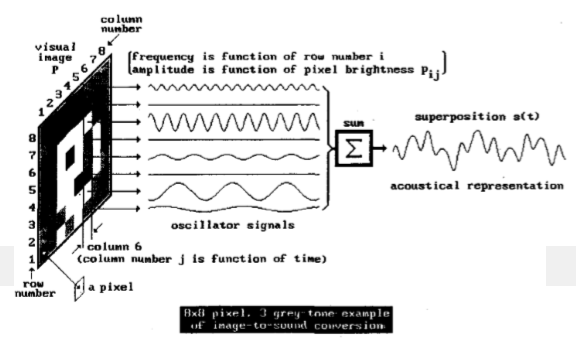
\includegraphics[width=1\textwidth]{image_to_sound}
\caption{\label{fig:image_to_sound}}
\end{figure}
  
The images have a resolution of 64 * 64 pixels with 16 gray-tones per pixels.  

The experiment showed promising functionality to convert images to sound but lacks a field study test on people with blindness. Moreover, the advantages and disadvantages of this system is yet to be proved. This questions the reliability of the system since there is no recordings of testing data presented in the article of the experiment. However theory supports the system's functionality. \todo{the math can be used in other projects}

\subsection{The Sound of Photographic Image}\label{sec:soundarticle}
\todo{most focus on point relevant for the project. please rework}

A use of photographic images for conversion into sound was performed and described in an article by Atau Tanaka, who is the chair of digital media and director of culture lab at Newcastle University.

The paper describes two processing methods that both converts image into sound.

The first method uses/utilises two !image/picture series! called "9m14s Over Vietman" and "Bondage" /*ved ikke om det er vigtigt at have navnene med*/. The method used to create the sound from the image, uses a temporary mapping and additive synthesis on raw grayscale images by scanning every pixel. A bright pixel produces high notes and a dark pixel produces a low note.

The second method was used for an interactive art installation. The interactive art consisted of a wooden structure with panels covered in rice paper to display Tanaka's pre-processed images from the "Bondage" !image/picture serie!. The images were processed through re-synthesis processes, where the frequency bands where quantisized to whole tones and pentatonic (was/were?) mapped in which the key notes are played one at a time. The images were projected with negative pixel values creating a inverted image of the original and each row displayed different frequency ranging from !sub-low! to high frequencies. An example of this result can be seen in the !figure/image! below. /*continue with ther stiff with the infrared cam*/


The project was based on three different photographic works, two of them were released on CD while the third was an interactive art installation with constantly changing images in collaboration with sound. The technical methods used to create the sound in the first "work" used a temporary mapping and additive synthesis on raw grayscale images, by scanning every pixel, whereas a very bright pixel produces high notes and opposite if the pixels are dark. 

The interactive art consisted of a wooden structure with panels covered in rice paper to display Tanaka's preprocessed images from the bondage source. The images were processed through resynthesis processes where the frequency bands where quantisized to whole tones and pentatonic mapped in which the key notes are played one at a time. The images were projected with negative pixel values creating a inverted image of the original and each row displayed different frequency ranging from sub-low to high frequencies. An example of this result can be seen in the figure below. 

(figure 5)

To capture human interaction, a infrared camera on top of the structure used viewers silhouettes as a layer on the negative image which uncovered the original black and white image as seen in the figure 6.

(figure 6)

This interaction also affected the produced sound which were based on the brightness and thus make new harmonies of sound. 

(Conclusion på artikel)
This visualisation of sound through images shows dynamic functionality of a interactive system, which utilize human interaction to /*alter?*/ the alteration of a preprossed image. However, since no data is presented of an evaluation of this exhibit, it is difficult to make a further development of this system. The authors reason for this system has been produced on the background of being a visual art. /* vi skal lige være sikker på den her påstand*/   
 

\section{Methods used to evaluate}\label{sub:methodsusedtoevaluate}






\section{State of the art}\label{sec:stateart}

\subsection{Sonic Photo}\label{sub:sonic}
\todo{make into reference}
Can be found here: http://www.skytopia.com/software/sonicphoto/

Sonic photo is a program that allows the user to transform an image into sound. The user can load an image into the program, and adjust various parameters to modify the resulting audio. The parameters include  frequency(Hz), brightness, tone, harmony quantization, etc.

\todo{more general information about the program. Which points to we want to make, by writing about this program?}